\chapter{Experiments} \label{chapter:experiments}

The following section describes the setups of the experiments conducted with the neural network presented in Chapter \ref{chapter:semi_automatic}. Due to the lack of existing annotated medical data, the focus of the experiments is to ascertain a network design and mode of operation that compensates this as best as possible. First, we test the different network architectures that were described in section \ref{section:network_variations} using the same parameters. We then choose the best architecture for further experiments which we use to evaluate the two different training schemes introduced in section \ref{section:modes_of_operation}: training from scratch and incremental training. The results are analyzed to an extend that is necessary to understand subsequent experiments but the in-depth discussion follows in Chapter \ref{chapter:discussion}.

\section{Terminology}

\noindent\textbf{Hyper-Parameter.} \textit{Hyper-parameters} are the tunable parameters of a network. The number and kind of parameters vary with the used type of network architecture, optimizer, etc.

\section{Datasets} \label{section:experiments_datasets}

\begin{figure}[!tbp]
	\centering
	\begin{subfigure}[t]{0.47\textwidth}
		\centering
    	\includegraphics[width=0.6\linewidth]{tless_example_train}
    	\caption{An example frame from the training dataset of T-Less.}
    	\label{fig:tless_example_train}
	\end{subfigure}
	\hfill
	\begin{subfigure}[t]{0.47\textwidth}
		\centering
    	\includegraphics[width=0.7\linewidth]{tless_example_test}
    	\caption{An example frame from the test dataset of T-Less.}
    	\label{fig:tless_example_test}
	\end{subfigure}
	\caption{Example frames from the T-Less dataset \cite{tless}.}
	\label{fig:tless_examples}
\end{figure}

The initial intention to completely annotate the medical images of the \ac{evc} dataset turned out to be not feasible (see Chapter \ref{chapter:manual_annotation}). Instead, we chose the T-Less dataset to conduct the experiments with. Its objects are mostly texture-less  and of rather small size, making them similar to surgical tools. Next to many human pose estimation datasets, there exist some datasets of objects, too, like \cite{next_view_dataset}, \cite{pracsys_dataset} and \cite{rigid_body_dataset}. But the objects of T-Less resemble surgical tools more than the objects of those datasets.

The T-Less dataset was released in 2017 by Hoda\v{n} et al. \cite{tless}. It contains the object models of 30 industry-relevant real world objects. Two versions exist: one mesh of the object that was manually reconstructed using CAD software and one that was produced from RGB-D images. The 3D coordinates of the objects reflect their size in millimeters. For example, the minimum and maximum of any component of the coordinates of object model 01 are about -30 and 30. This means that the model is about 60 mm long. The objects were captured using a Primsense CARMINE 1.09, a Microsoft Kinect v2 and a Canon IXUS 950 IS. We used the photos of the Canon camera due to their quality and since we do not need depth information, which is also provided by the CARMINE sensor and the Kinect. There are 1296 images of each object in the training set of the dataset, sampled in 10 degree steps in elevation and 5 degree azimuth. 20 test scenes, consisting of 504 images each, exist as well. Those are photographs of cluttered scenes of different complexity, with sometimes more than 15 objects visible. All training and test images are annotated with the ground-truth poses of the visible objects. The authors also provide a tool set to render the objects at a given pose. \fig \ref{fig:tless_example_train} shows an example frame from the training set and \fig. \ref{fig:tless_example_test} an example frame from the test set. The training images of the other objects look similar to the depicted image. The dataset provides depth images, as well but this is irrelevant to our setting.

\section{Data Preparation}

The T-Less dataset does neither provide 3D object coordinates nor segmentation masks. This is the reason why we rendered both ourselves. The rendering script is part of the network package. Because the 16-bit TIFF object coordinate ground-truth files used up too much disk space when kept in their original size, they were cropped to the relevant area by determining the smallest box around the segmentation pixels. The images and segmentation masks were cropped to the same area and the camera matrices adjusted accordingly. We used 16-bit TIFF files instead of 32-bit because we deemed the accuracy of 16-bit to be high enough.

\section{Evaluation Metric}

We developed a set of evaluation metrics to capture different aspects of the prediction quality of a network. We assumed that multiple metrics provide better insights of the strengths and weaknesses of an architecture. To this end, we provide functionality that directly assesses the quality of the predicted object coordinates and also functionality that provides details on the accuracy of the resulting recovered pose.

The \textit{Object Coordinate Error} $e_{\text{coord}}$ computes the euclidean distances between the predicted and ground-truth object coordinates:
\begin{align*}
e_{\text{coord}} = \frac{1}{|S_O|} \sum\limits_{(i, j)} \sqrt{(g_{ij1} - p_{ij1})^2 +(g_{ij2} - p_{ij2})^2 + (g_{ij3} - p_{ij3})^2}
\end{align*}
where $(i, j)$ are all 2D locations belonging to the object model $O$ according to the segmentation mask. $|S_O|$ denotes the cardinality of the set of these locations. $g_{ijk}$ and $p_{ijk}$ are the $k$-th components of the object coordinate at $(i, j)$ in the ground-truth and predicted object coordinates image, respectively.

The number of \textit{Inliers} $n_{\text{inlier}}$ captures the number of object coordinates whose euclidean distance to the ground-truth object coordinate is below a certain threshold:
\begin{align*}
e_{\text{inlier}} = \left\rvert\left\lbrace(i,j) \ \bigg| \ \sqrt{(g_{ij1} - p_{ij1})^2 +(g_{ij2} - p_{ij2})^2 + (g_{ij3} - p_{ij3})^2} \leq \sigma_{\text{thresh}}\right\rbrace \right\rvert
\end{align*}
where $\sigma_{\text{thresh}}$ is the chosen threshold and $(i,j)$ are all locations belonging to the object model. We set the threshold to 2.

Both $e_{\text{coord}}$ and $n_{\text{inlier}}$ assess the accuracy of the predicted object coordinates. The metrics described next provide a measure of the quality of the recovered pose.

The \textit{Distance Error} $e_{\text{dist}}$ is the euclidean distance between the ground-truth position of the object and the position computed by \ac{ransac}. $e_{\text{dist}}$ is computed as:
\begin{align*}
e_{\text{dist}} = \sqrt{(t_{g1} - t_{p1})^2 +(t_{g2} - t_{p2})^2 + (t_{g3} - t_{p3})^2}
\end{align*}
where $t_{gk}$ denotes the $k$-th component of the ground-truth translation vector, and $t_{pk}$ the $k$-th component of the translation vector recovered from the coordinate predictions.

The \textit{Angle Error} $e_{\text{angle}}$ is the rotational error in degrees between the ground-truth and the calculated rotation matrix:
\begin{align*}
e_{\text{angle}} = \frac{cos^{-1}(\frac{\Tr(R_g^TR_p) - 1}{2}) \cdot 180\degree}{\pi}
\end{align*}
where $R_g$ and $R_p$ denote the ground-truth and predicted rotation matrix, respectively and $Tr()$ denotes the trace of a matrix.

Finally, we implemented the metric presented by Hinterstoisser \etal in \cite{hinterstoisser2}, which computes the average distance between each vertex of the object model with the ground-truth and recovered pose applied to it. This metric $e_{\text{pose}}$ is defined in the following way:
\begin{align*}
e_{\text{pose}} = \frac{1}{|M|} \sum\limits_{X \in M}||(\bar{R}X + \bar{t}) - (RX + t)||
\end{align*}
where $M$ is the set of points of an object model $O$. $\bar{R}$ and $\bar{t}$ denote the rotation matrix and translation vector of the ground-truth pose $\bar{P}$, while $R$ and $t$ are the respective components of the recovered pose. A pose is an \textit{inlier}, if
\begin{align*}
e_{\text{pose}} \leq khs \cdot d
\end{align*}
where $d$ is the diameter of the object and $khs$ is a constant which we set to $0.1$ for the rest of this work. The percentage of inliers is denoted as \textit{inlier \%} in the tables of the experiments.

The scripts that we provide compute various partitions of the metrics. Next to the mean for all five metrics, the median at 25, 50 and 75\% is calculated for each metric individually, as well. This makes it easier to assess whether a network produces inaccurate predictions for only a part of the dataset. We only provide the mean values in this chapter though because using the median for comparison requires to compare at least all three medians computed by the script. Otherwise, anomalies can occur. For example, the pose inlier rate can only be computed as the average over all images which, in some rare cases, contradicts the result of comparing the median at 50 \% metrics of different networks.

\section{Training Experiments}

This section describes the configuration of the different training experiments. First, we compare the SGD and Adam optimizer in \ref{subsection:optimizers}. Then, we evaluate the different architectures in \ref{subsection:architectures}. Finally, we asses training from scratch and incremental training in Section \ref{subsection:experiments_online_learning}. We conducted all experiments on the object model $01$ of the T-Less dataset. The image dimension was set to 500 pixels (for width and height), which is larger than the largest area covering an object in any image. All experiments were run using the training data of the object model $01$. For some experiments we only used a subset of the available images (see Sections \ref{subsection:experiments_online_learning} and \ref{subsection:experiments_active_learning}) but we always split the data into 70\% training images and 30\% validation images. The images were assigned to one of the sets at random. If not stated otherwise, we used the same training and validation set throughout the experiments. The axis labeled \textit{epochs} in the loss graphs denotes the number of epochs the training was run for. Each epoch consisted of 1000 iterations in every experiment.

\begin{table}[]
\centering
\begin{tabular}{|l||lllll|}
\hline
Run                                                     & 1     & 2      & 3       & 4        & 5         \\ \hline \hline
\rowcolor{Gray}
Epochs                                                  & 30    & 45     & 55      & 65       & 70        \\
\begin{tabular}[c]{@{}l@{}}Learning\\ Rate\end{tabular} & 0.001 & 0.0001 & 0.00001 & 0.000001 & 0.0000001 \\  \hline
\end{tabular}
\caption{The configuration of the SGD optimizer used in the experiment to compare SGD and Adam.}\label{table:experiments_optimizers_sgd}
\end{table}

\subsection{Optimizers} \label{subsection:optimizers}  

\begin{figure}[!tbp]
	\begin{subfigure}[t]{0.4\textwidth}
			\begin{tikzpicture}[scale=0.95]
  				\begin{axis}[cycle list name=tb, 
                 grid=both,
                 grid style={solid,gray!30!white},
                 axis lines=middle,
    			 xmin = 0,
    			 xmax = 60,
    			 ymin = 0,
    			 ymax = 9,
                 xlabel={epoch},
                 ylabel={loss},
                 x label style={at={(axis description cs:0.5,-0.1)},anchor=north},
                 y label style={at={(axis description cs:-0.1,.5)},rotate=90,anchor=south},]
      			\addplot[smooth,tb_color_1] table [x=Step, y=Value, col sep=comma] {experiments/model1/exp1_adam_l1/train_loss.csv};
      			\addplot[smooth,tb_color_2] table [x=Step, y=Value, col sep=comma] {experiments/model1/exp1_sgd/train_loss.csv};
      			\addlegendentry{Adam}
				\addlegendentry{SGD}
    			\end{axis}
			\end{tikzpicture}
		\caption{Training losses.}
	\end{subfigure}
	\hspace{15mm}
	\begin{subfigure}[t]{0.4\textwidth}
			\begin{tikzpicture}[scale=0.95]
  				\begin{axis}[cycle list name=tb, 
                 grid=both,
                 grid style={solid,gray!30!white},
                 axis lines=middle,
    			 xmin = 0,
    			 xmax = 60,
    			 ymin = 0,
    			 ymax = 9,
                 xlabel={epoch},
                 ylabel={loss},
                 x label style={at={(axis description cs:0.5,-0.1)},anchor=north},
                 y label style={at={(axis description cs:-0.1,.5)},rotate=90,anchor=south},]
      			\addplot[smooth,tb_color_1] table [x=Step, y=Value, col sep=comma] {experiments/model1/exp1_adam_l1/val_loss.csv};
      			\addplot[smooth,tb_color_2] table [x=Step, y=Value, col sep=comma] {experiments/model1/exp1_sgd/val_loss.csv};
      			\addlegendentry{Adam}
				\addlegendentry{SGD}
    			\end{axis}
			\end{tikzpicture}
		\caption{Validation losses.}
	\end{subfigure}
	\caption{Training and validation losses of Adam and SGD used to train architecture 1. The plot is cropped on the $y$-axis to enhance the differences.}
	\label{fig:experiments_adam_sgd_loss}
\end{figure} 

To obtain the best optimizer for further experiments, we compared SGD and Adam using the first architecture we constructed. This architecture consists of 23 layers and has a receptive field-size of 99. The hyper-parameters $\beta_1$ and $\beta_2$ of the Adam optimizer were left at the default values set by Keras, which are $0.9$ and $0.999$, respectively. The more complex configuration of the SGD optimizer is given in Table \ref{table:experiments_optimizers_sgd}. Fig. \ref{fig:experiments_adam_sgd_loss} shows the loss of both experiments during training. The SGD optimizer profits from the reduction of the learning rate around epoch 30, visible as the small step in the training loss. This could imply that further tuning of the training parameters of SGD could lead to better results. But since the Adam optimizer does not need manual fine-tuning of its hyper-parameters and performs visibly better than SGD, we chose Adam as the optimizer for all following experiments. We based our conclusion that Adam is the superior optimizer for our network solely on the loss values. Since we trained the same network architecture twice and only varied the optimizers, better error rates mean better overall results.

\subsection{Loss Functions}

\begin{table}[]
\centering
\begin{tabular}{|l||llllll|}
\hline 
 Loss  & $e_{\text{coord}}$ & $n_{\text{inlier}}$ & $e_{\text{angle}}$ & $e_{\text{dist}}$  & $e_{\text{pose}}$ & inlier \%  \\ \hline \hline \rowcolor{Gray}
L1 & \textbf{1.6494} & \textbf{569.4318} & \textbf{1.6416} & \textbf{5.4331} & \textbf{5.4627} & \textbf{78.92} \\
L2 & 1.5429    & 546.5629    & 2.0507      & 6.2401 & 6.2713 & 70.17 \\ \hline   
\end{tabular}
\caption{The metrics on the \textbf{validation set} of the experiments comparing the loss functions.}
\label{table:experiments_loss_functions}
\end{table}

To prove our statement that the L1 loss is more suitable than the L2 loss for our application, we conducted another training run using the L2 loss and compared it to the run using the L1 loss of the previous experiment. The loss function comparisons are depicted in Appendix \ref{fig:experiments_l1_l2_loss} but are omitted here, due to their limited comparability. To obtain the L2 loss, we removed taking the square root from the loss function which naturally results in higher error rates. Table \ref{table:experiments_loss_functions} shows the metrics of the experiments with the different loss functions. The L1 loss offers superior accuracy and is used in all further experiments.

\begin{figure}[!tbp]
	\begin{subfigure}[t]{0.47\textwidth}
		\centering
    	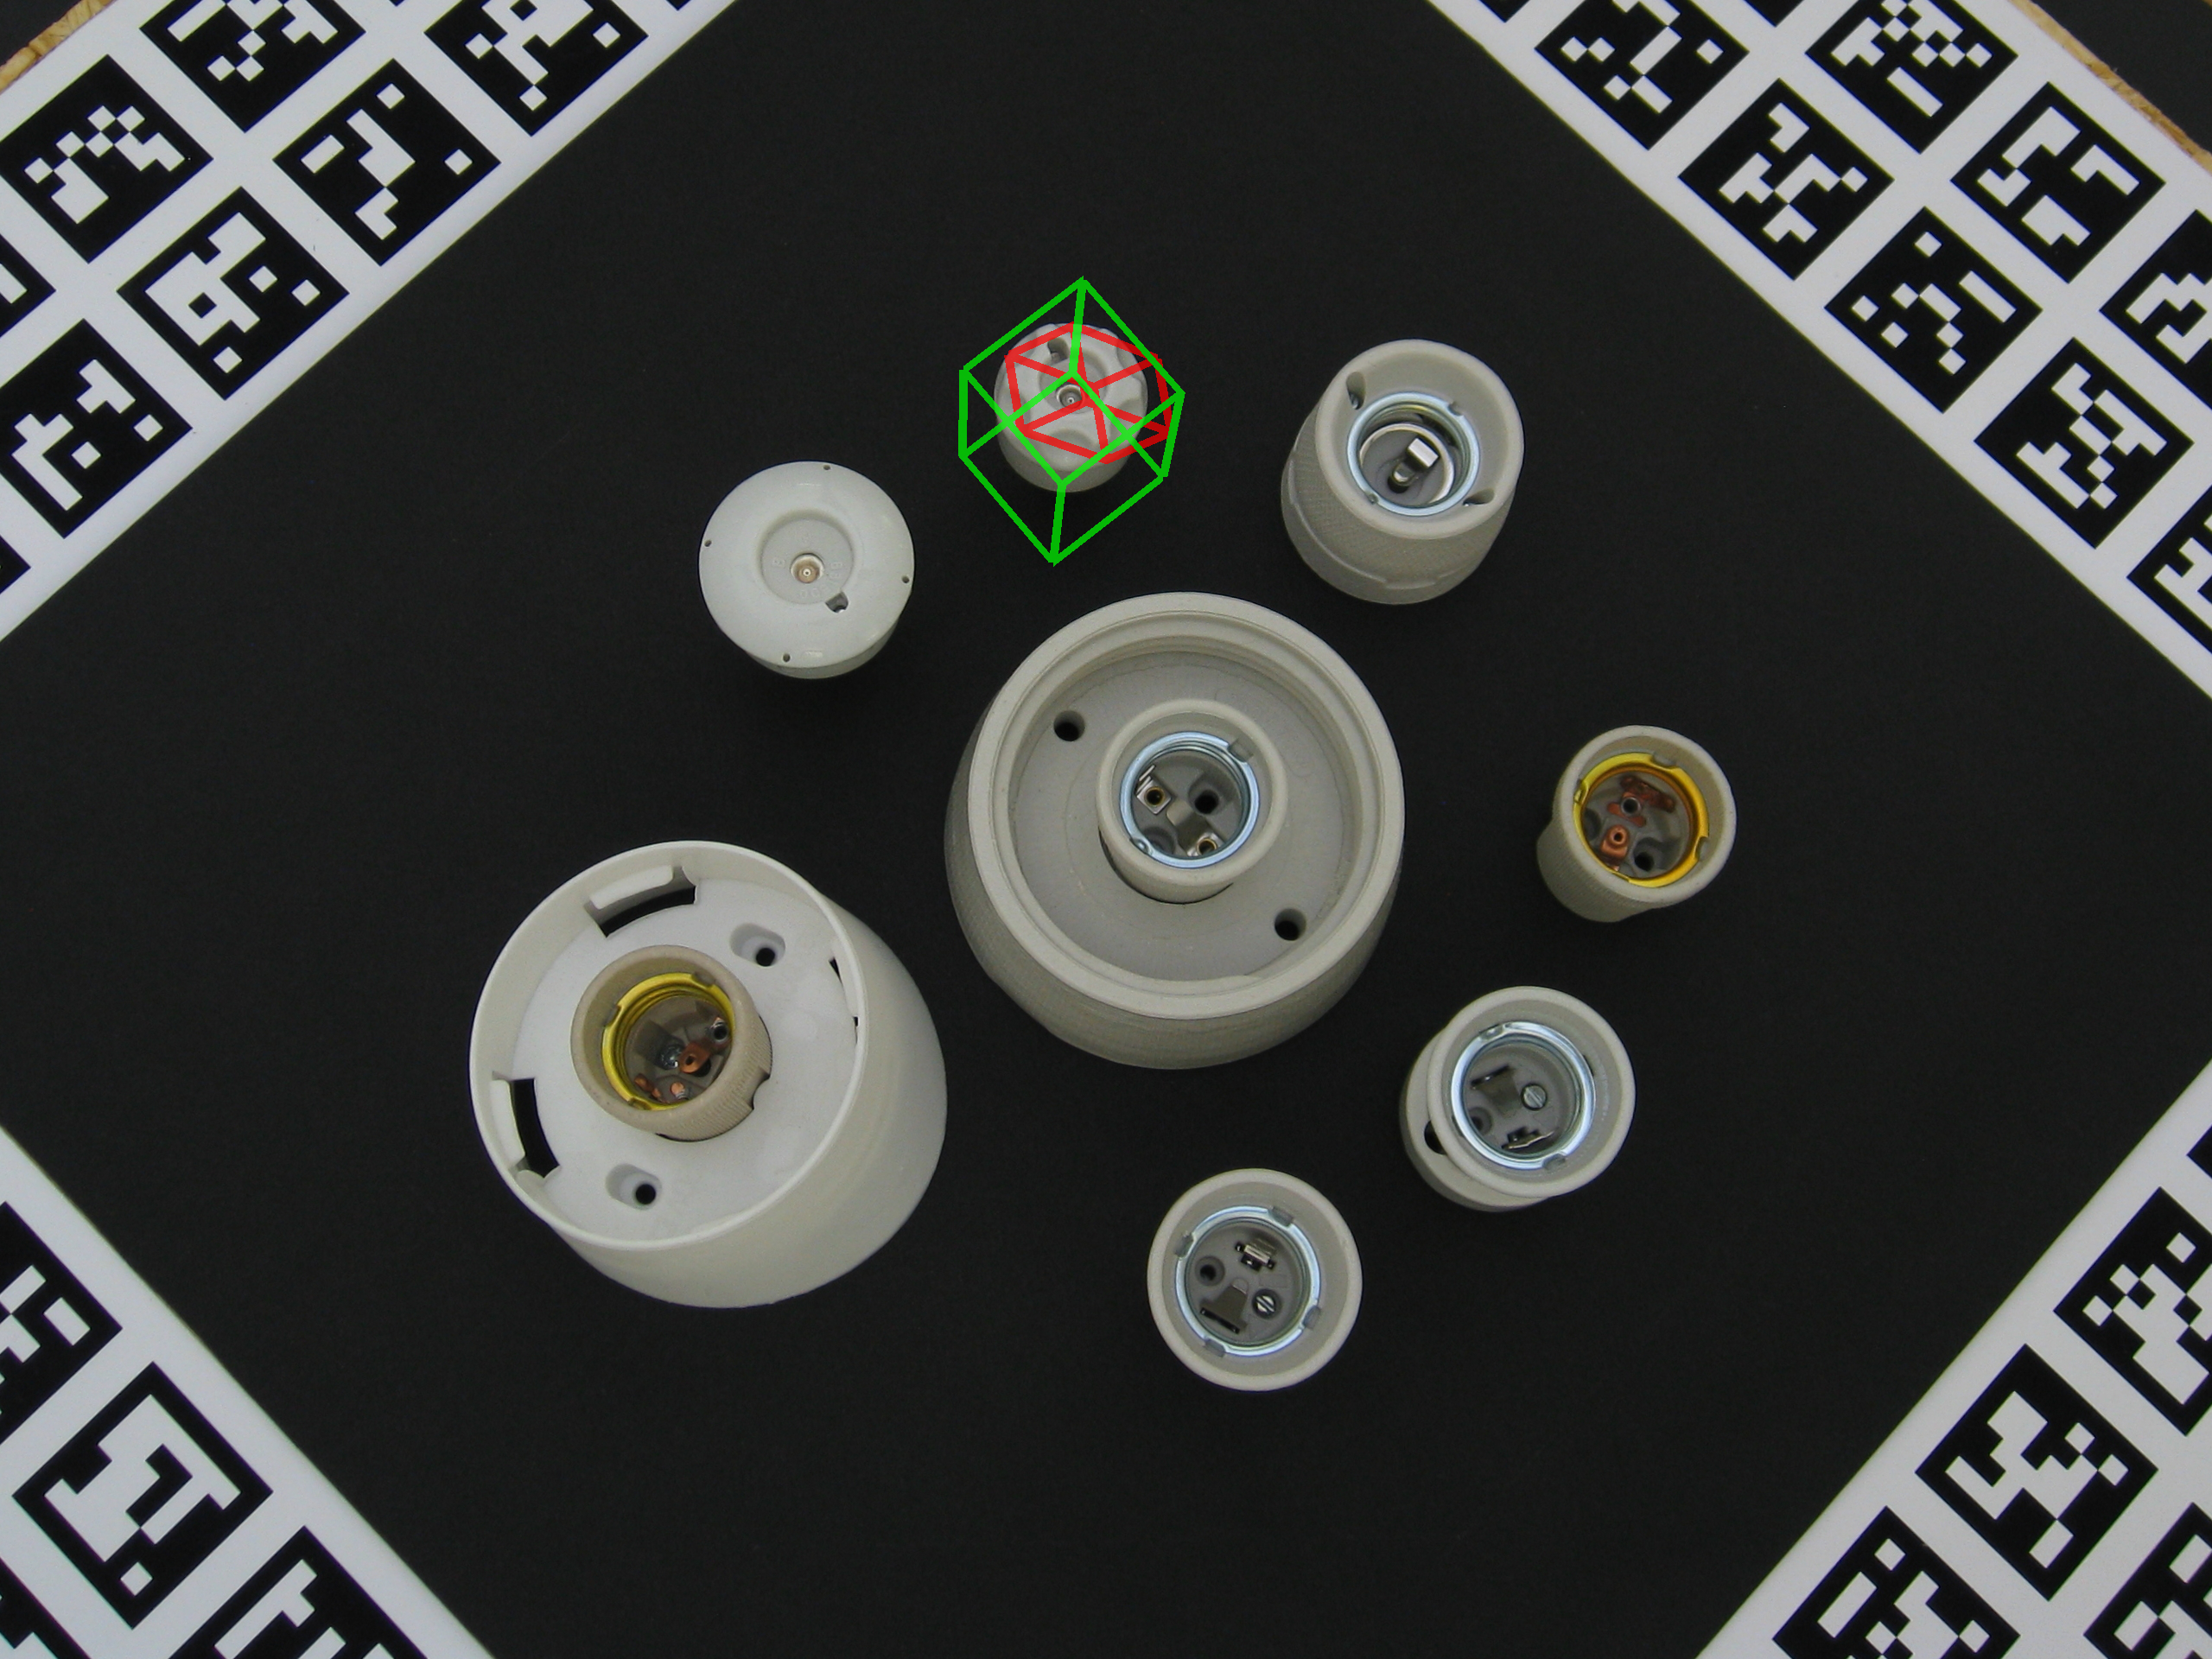
\includegraphics[width=0.7\linewidth]{experiments/model1/0045_bounding_boxes}
    	\caption{Image 0045.jpg with inferred poses.}
	\end{subfigure} 
	\hfill
	\begin{subfigure}[t]{0.47\textwidth}
		\centering
    	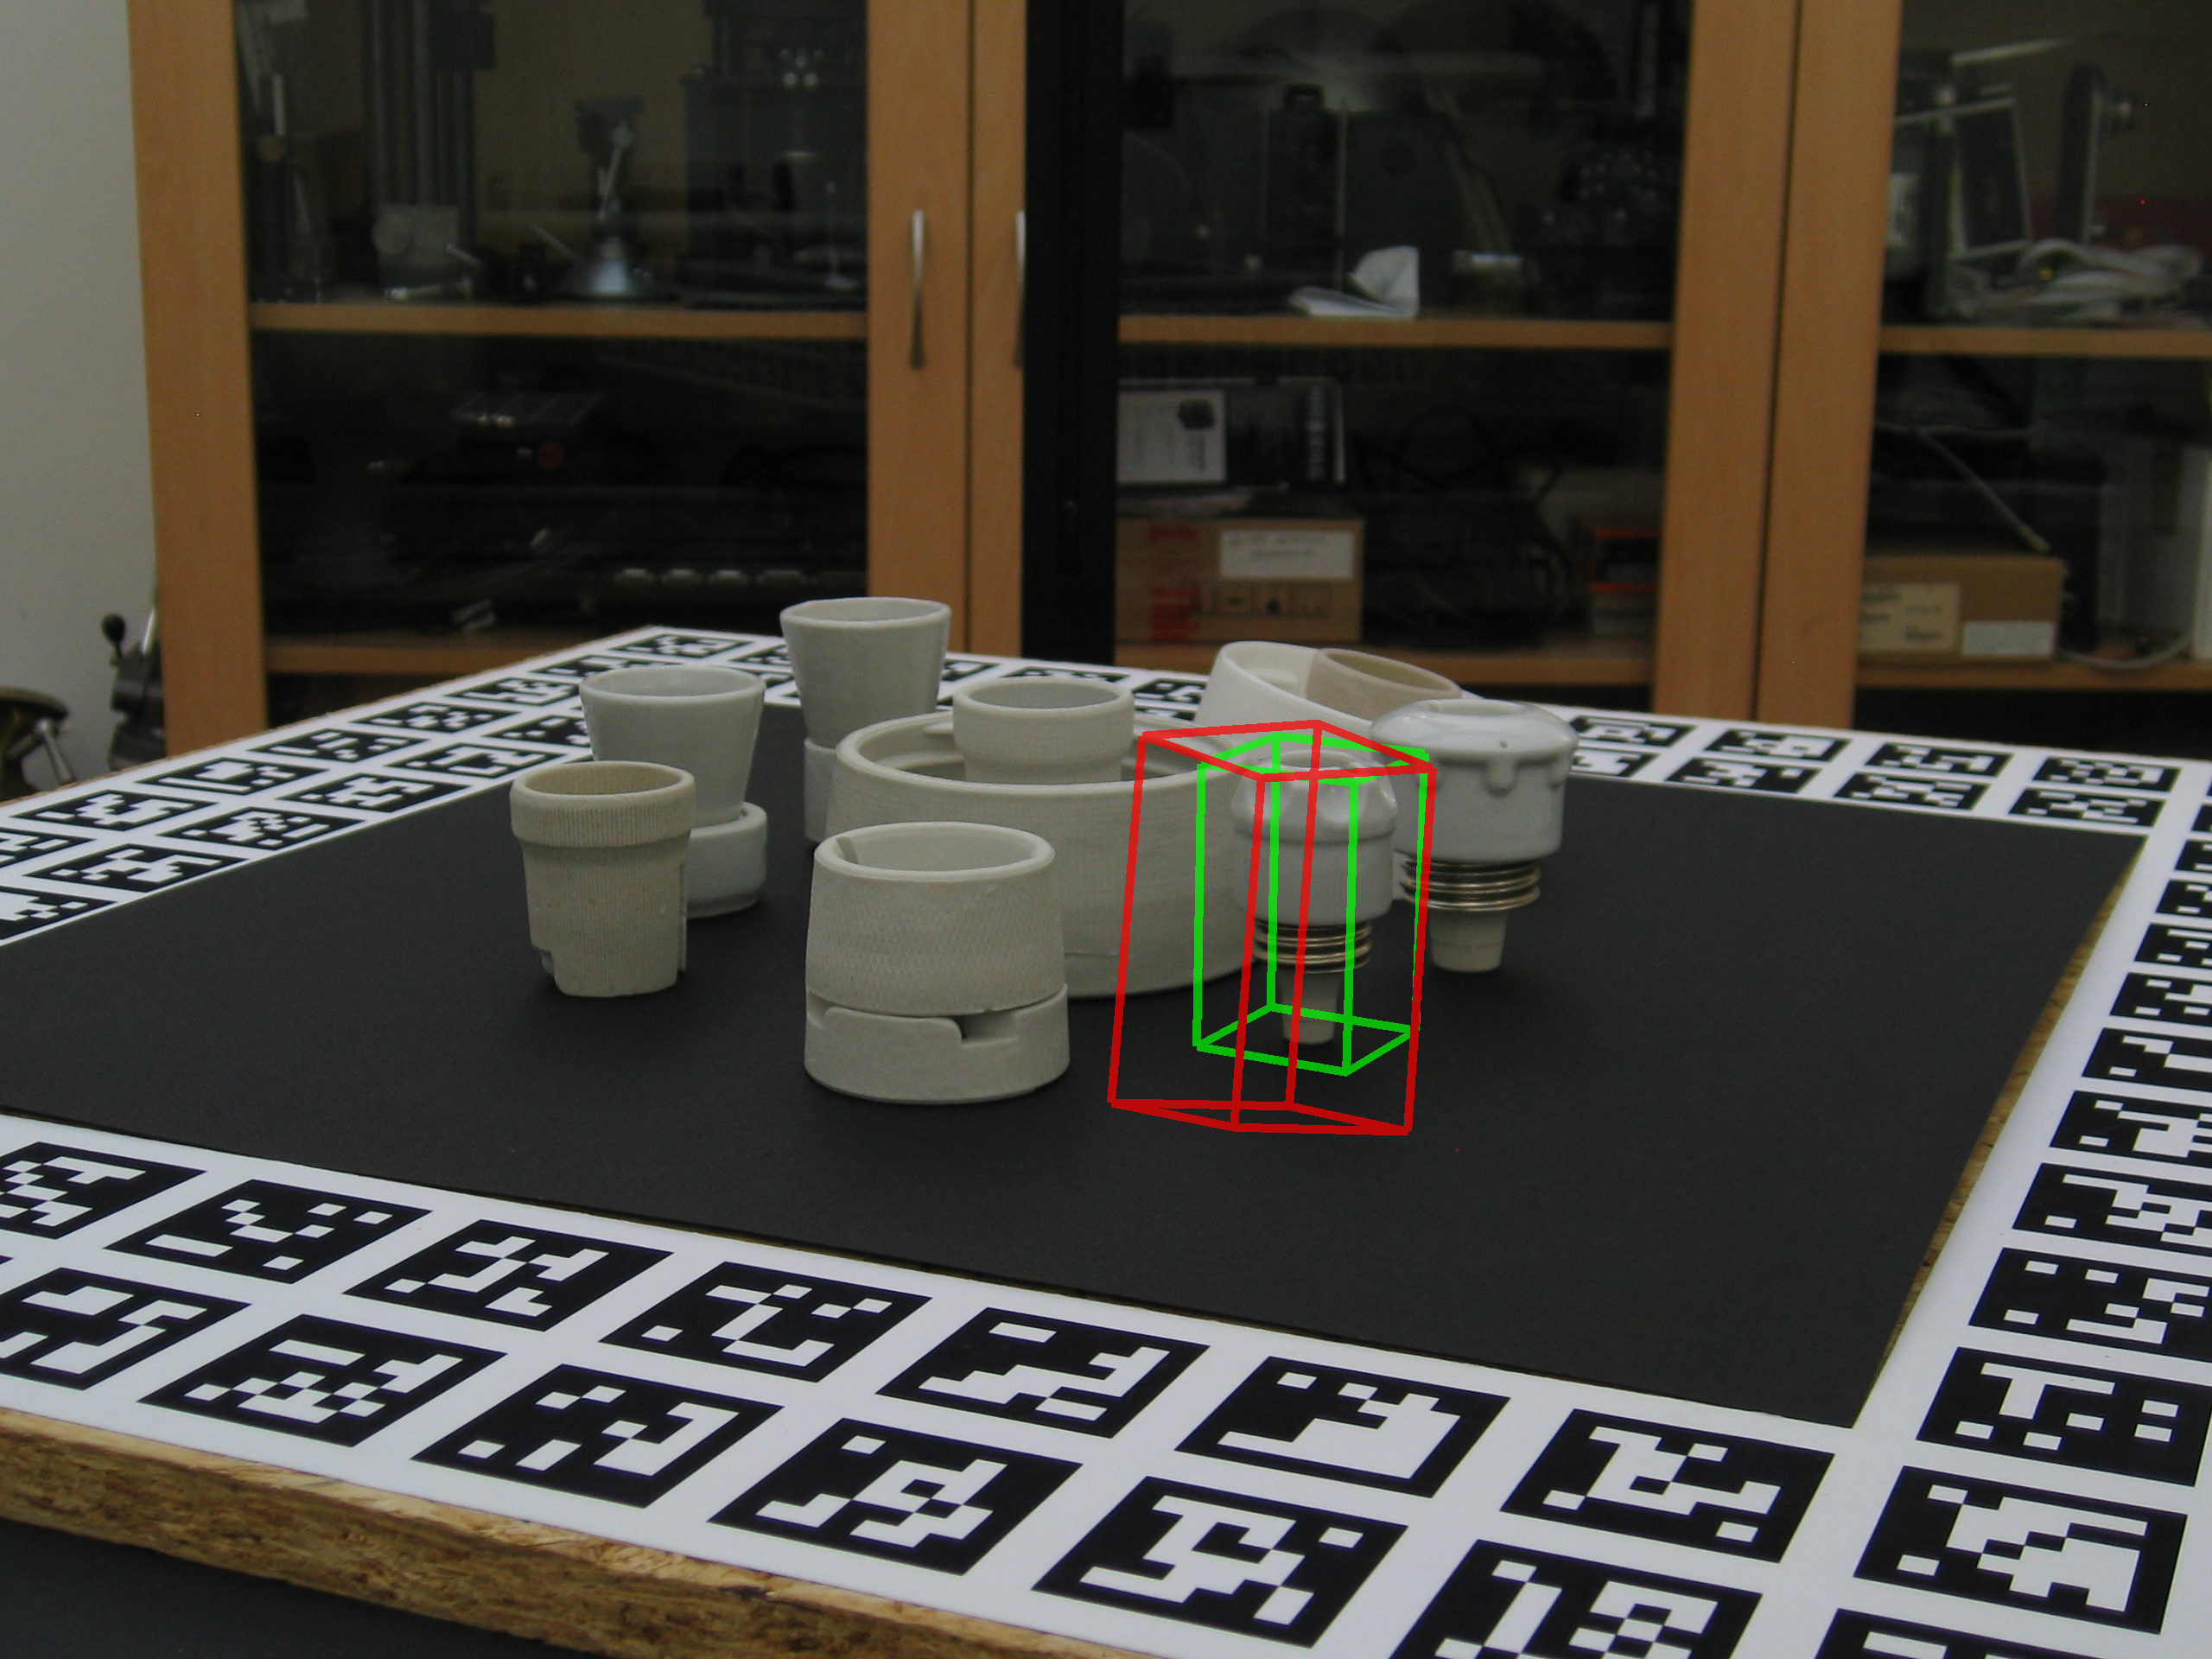
\includegraphics[width=0.7\linewidth]{experiments/model1/0438_bounding_boxes}
    	\caption{Image 0438.jpg with inferred poses.}
	\end{subfigure} 
	\caption{Example images from test scene 7 of the T-Less dataset with poses inferred by architecture 1 trained on all images. The green bounding box was derived from the ground-truth pose, the red bounding box from the predicted pose.}
	\label{fig:architecture_experiments_example_frames}
\end{figure} 

\subsection{Architectures} \label{subsection:architectures}

\begin{figure}[!tbp]
	\begin{subfigure}[t]{0.4\textwidth}
			\begin{tikzpicture}[scale=0.95]
  				\begin{axis}[cycle list name=tb, 
                 grid=both,
                 grid style={solid,gray!30!white},
                 axis lines=middle,
                 xlabel={epoch},
    			 xmax = 70,
    			 ymax = 8,
                 ylabel={loss},
                 x label style={at={(axis description cs:0.5,-0.1)},anchor=north},
                 y label style={at={(axis description cs:-0.1,.5)},rotate=90,anchor=south},]
      			\addplot[smooth,tb_color_1] table [x=Step, y=Value, col sep=comma] {experiments/model1/exp1_adam_l1/train_loss.csv};
      			\addplot[smooth,tb_color_2] table [x=Step, y=Value, col sep=comma] {experiments/model2/train_loss.csv};
      			\addplot[smooth,tb_color_3] table [x=Step, y=Value, col sep=comma] {experiments/model3/train_loss.csv};
      			\addplot[smooth,tb_color_4] table [x=Step, y=Value, col sep=comma] {experiments/model4/train_loss.csv};
      			\addplot[smooth,tb_color_5] table [x=Step, y=Value, col sep=comma] {experiments/model5/exp1/train_loss.csv};
      			\addplot[smooth,tb_color_6] table [x=Step, y=Value, col sep=comma] {experiments/model6/train_loss.csv};
      			\addlegendentry{Architecture 1}
				\addlegendentry{Architecture 2}
				\addlegendentry{Architecture 3}
				\addlegendentry{Architecture 4}
				\addlegendentry{Architecture 5}
				\addlegendentry{Architecture 6}
    			\end{axis}
			\end{tikzpicture}
		\caption{Training losses.}
	\end{subfigure}
	\hspace{15mm}
	\begin{subfigure}[t]{0.4\textwidth}
			\begin{tikzpicture}[scale=0.95]
  				\begin{axis}[cycle list name=tb, 
                 grid=both,
                 grid style={solid,gray!30!white},
                 axis lines=middle,
                 xlabel={epoch},
    			 xmax = 70,
    			 ymax = 8,
                 ylabel={loss},
                 x label style={at={(axis description cs:0.5,-0.1)},anchor=north},
                 y label style={at={(axis description cs:-0.1,.5)},rotate=90,anchor=south},]
      			\addplot[smooth,tb_color_1] table [x=Step, y=Value, col sep=comma] {experiments/model1/exp1_adam_l1/val_loss.csv};
      			\addplot[smooth,tb_color_2] table [x=Step, y=Value, col sep=comma] {experiments/model2/val_loss.csv};
      			\addplot[smooth,tb_color_3] table [x=Step, y=Value, col sep=comma] {experiments/model3/val_loss.csv};
      			\addplot[smooth,tb_color_4] table [x=Step, y=Value, col sep=comma] {experiments/model4/val_loss.csv};
      			\addplot[smooth,tb_color_5] table [x=Step, y=Value, col sep=comma] {experiments/model5/exp1/val_loss.csv};
      			\addplot[smooth,tb_color_6] table [x=Step, y=Value, col sep=comma] {experiments/model6/val_loss.csv};
    			\end{axis}
			\end{tikzpicture}
		\caption{Validation losses.}
	\end{subfigure}
	\caption{Training and validation losses of the different architectures. The $y$ axis is cropped to enhance the more delicate differences at the lower end. The validation losses of architectures 4 and 6 are too high to be displayed here.}
	\label{fig:experiments_architectures_loss}
\end{figure} 

\begin{table}[b]
\centering
\begin{tabular}{|l||llllll|} \hline
Architecture & $e_{\text{coord}}$ & $n_{\text{inlier}}$ & $e_{\text{angle}}$ & $e_{\text{dist}}$ & $e_{\text{pose}}$ & inlier \% \\ \hline \hline \rowcolor{Gray}
1            & \textbf{1.6494}    & \textbf{569.4318}   & 1.6416             & 5.4331   & 5.4627      & 78.92  \\ \hline
2            & 3.0175             & 482.0385            & 6.2531             & 14.1186            & 14.3991    & 77.3778       \\ \hline \rowcolor{Gray}
3            & 4.5000             & 322.1516            & 5.2395             & 11.0992            & 11.2473    & 59.8971        \\ \hline
5            & 2.3125             & 510.7506            & \textbf{1.1989}    & \textbf{2.4177}    & \textbf{2.4640}     & \textbf{97.6863} \\ \hline       
\end{tabular}
\caption{The evaluation metrics on the \textbf{validation set} of architectures 1 - 3 and 5, which were trained using all available images.}
\label{table:architecture_validation_metrics_comparison}
\end{table}

The experiments with the different architectures were all performed using the Adam optimizer with the parameters mentioned in Section \ref{subsection:optimizers} and the L1 loss.
Therefore, the only difference is the used architecture. The losses of the experiments are displayed in \fig \ref{fig:experiments_architectures_loss}. Two example images from test scene 7 of the T-Less dataset with rendered bounding boxes of the poses inferred by architecture 1 are shown in \fig \ref{fig:architecture_experiments_example_frames}. The same images with poses inferred by architectures 2, 3 and 5 are provided in Appendix \ref{fig:appendix_architecture_comparison_example_frames}. The images show the issue of the increased rotational error when an image shows a view of an object along the $z$-axis. The sideways view allows the network to predict poses more accurately. This issue can be seen in the error image of \fig \ref{fig:architecture_comparison_errors}. An error image of a perfect prediction would be completely black. The top-down view shows a lot of bright colors, which implies high errors.

The largest gap of the losses is between architectures 4 and 6 and the four remaining architectures. This gap is especially large in the validation loss but also observable in the training loss. Architectures 4 and 6 employ dropout, as opposed to architectures 1 - 3 and 5, which use batch normalization (with batch sizes of 14, 10, 14 and 3, respectively). The authors of \cite{batch_normalization}  propose that batch normalization reaches better optima than dropout, which could explain the training loss difference. The validation losses of the two dropout architectures actually increase, which is not visible in the graph. This indicates that the networks overfit to the data. The constantly increasing validation loss is the reason why we did not keep the training processes of architectures 4 and 6 running, despite their training errors still decreasing. Proper exploration of hyper-parameters, like frequency of the dropout layers, as well as the dropout frequency itself, could improve the performance of architectures 4 and 6. But since batch normalization achieves a good accuracy without further fine-tuning, we did not investigate these architectures any further.

The metrics of architectures 1 - 3 and 5 are provided in Table \ref{table:architecture_validation_metrics_comparison}. Architecture 5 performs best, followed by architecture 1. The table shows that multiple different metrics can give a deeper grasp of a network's performance, as architecture 1 has a significantly lower object coordinate error ($e_{\text{coord}}$) than architecture 5 but their pose errors ($e_{\text{pose}}$) are of similar quality. Architecture 2 offers a better object coordinate error than architecture 5 but achieves a worse pose error.

The results of the training experiments of the different architectures lead us to choose architectures 1 and 5 for further experiments, i.e. a shallower architecture with larger receptive field-size and a deeper architecture with reduced receptive field-size. Table \ref{table:architecture_test_metrics_comparison} shows the evaluation metrics for the networks on test scene 7 of the T-Less dataset. Architectures 1 and 5 achieve the best accuracy which supports our decision to use them in the following experiments. In These experiments we investigate how the two different designs behave when trained with smaller datasets.

\begin{figure}[!tbp]
	\centering
	\vspace{5mm}
	\begin{subfigure}[t]{0.22\textwidth}
		\centering
    	\includegraphics[width=0.9\linewidth]{/experiments/model1/0040}
    	\caption{Image 0040.jpg.}
	\end{subfigure}
	\hfill
	\begin{subfigure}[t]{0.22\textwidth}
		\centering
    	\includegraphics[width=0.9\linewidth]{/experiments/model1/0040_obj_coords_error}
    	\caption{The corresponding error of the object coordinate prediction on image 0040.jpg made by architecture 1.}
	\end{subfigure}
	\begin{subfigure}[t]{0.22\textwidth}
		\centering
    	\includegraphics[width=0.5\linewidth]{/experiments/model1/0575}
    	\caption{Image 0575.jpg.}
	\end{subfigure}
	\hfill
	\begin{subfigure}[t]{0.22\textwidth}
		\centering
    	\includegraphics[width=0.5\linewidth]{/experiments/model1/0575_obj_coords_error}
    	\caption{The corresponding error of the object coordinate prediction on image 0575.jpg made by architecture 1.}
	\end{subfigure}
	\caption{Example training images from the T-Less dataset and the error of the object coordinate predictions of architecture 1 which was trained on all images. Bright colors imply a high error. The error was computed as the absolute difference between the ground-truth and predicted XYZ components. In the optimal case the error image would be black. A view along the $z$-axis impose a problem that is more difficult.}
	\label{fig:architecture_comparison_errors}
\end{figure}

\begin{table}[t]
\centering
\begin{tabular}{|l||llllll|} \hline
Architecture & $e_{\text{coord}}$ & $n_{\text{inlier}}$ & $e_{\text{angle}}$ & $e_{\text{dist}}$ & $e_{\text{pose}}$ & inlier \% \\ \hline \hline \rowcolor{Gray}
1            & 13.9062            & 60.7162   & 67.7789   & 158.3841           & 160.7716             & 5.7539 \\ \hline
2            & 14.6875            & 55.8055   & 68.1237   & 183.78932          & 186.3252            & 4.7619           \\ \hline \rowcolor{Gray}
3            & 15.4296            & 31.7361   & 85.2801   & 262.3253           & 265.8469           & 0.7936         \\ \hline
5            & \textbf{9.2421}    & \textbf{161.6011}     & \textbf{49.4737}   & \textbf{119.0649}  & \textbf{120.8825} & \textbf{7.7380} \\ \hline       
\end{tabular}
\caption{The evaluation metrics on the \textbf{test set} of architectures 1 - 3 and 5, which were trained using all available images.}
\label{table:architecture_test_metrics_comparison}
\end{table}

\subsection{Incremental Training} \label{subsection:experiments_online_learning}

To propose a training strategy that makes optimal use of the little data available at the beginning of manually annotating an unannotated dataset, we investigate here whether the network should be trained incrementally or from scratch. To this end, we trained architectures 1 and 5 incrementally with datasets consisting of 25 images. Thus, we trained the network using 25 images and then continued to train it with the next set of 25 images. We repeated this process until we reached 250 images. We used a maximum of 250 images in the incremental experiments because we deemed the incremental approach to be most relevant in this range. As we assumed that the proportion of the split of training and validation set becomes more relevant for such a small dataset, we ran one set of experiments using 70\% of the images for training (i.e. 18 images) and 30\% for validation (i.e. 7 images) and another set using a 90/10 split (22 images for training and 3 images for validation). The experiments utilizing the 70/30 split used the validation images of previous experiments for validation again, while the experiments of the 90/10 split did not. None of the training runs used training images of the previous experiments again.

\begin{figure}[!tbp]
	\begin{subfigure}[t]{0.4\textwidth}
			\begin{tikzpicture}[scale=0.95]
  				\begin{axis}[cycle list name=tb, 
                 grid=both,
                 grid style={solid,gray!30!white},
                 axis lines=middle,
                 xlabel={epoch},
                 xmax = 100,
    			 ymax = 8,
                 ylabel={loss},
                 x label style={at={(axis description cs:0.5,-0.1)},anchor=north},
                 y label style={at={(axis description cs:-0.1,.5)},rotate=90,anchor=south},]
      			\addplot[line width=2pt,dotted,tb_color_1] table [x=Step, y=Value, col sep=comma] {experiments/model1/exp7_25/train_loss.csv};
      			\addplot[line width=2pt,dotted,tb_color_2] table [x=Step, y=Value, col sep=comma] {experiments/model1/exp7_50/train_loss.csv};
      			\addplot[line width=2pt,dotted,tb_color_3] table [x=Step, y=Value, col sep=comma] {experiments/model1/exp7_100/train_loss.csv};
      			\addplot[line width=2pt,dotted,tb_color_4] table [x=Step, y=Value, col sep=comma] {experiments/model1/exp7_250/train_loss.csv};
      			\addplot[line width=1pt,smooth,tb_color_5] table [x=Step, y=Value, col sep=comma] {experiments/model1/exp3/train_loss.csv};
      			\addplot[line width=1pt,smooth,tb_color_6] table [x=Step, y=Value, col sep=comma] {experiments/model1/exp4/train_loss.csv};
      			\addplot[line width=1pt,smooth,tb_color_7] table [x=Step, y=Value, col sep=comma] {experiments/model1/exp5/train_loss.csv};
      			\addplot[line width=1pt,smooth,tb_color_8] table [x=Step, y=Value, col sep=comma] {experiments/model1/exp6/train_loss.csv};
				\addlegendentry{25 [inc 70/30]}
				\addlegendentry{50 [inc 70/30]}
				\addlegendentry{100 [inc 70/30]}
				\addlegendentry{250 [inc 70/30]}
				\addlegendentry{250}
				\addlegendentry{100}
				\addlegendentry{50}
				\addlegendentry{25}
    			\end{axis}
			\end{tikzpicture}
		\caption{70/30 training losses compared to training losses from scratch.}
	\end{subfigure}
	\hspace{15mm}
	\begin{subfigure}[t]{0.4\textwidth}
			\begin{tikzpicture}[scale=0.95]
  				\begin{axis}[cycle list name=tb, 
                 grid=both,
                 grid style={solid,gray!30!white},
                 axis lines=middle,
                 xlabel={epoch},
    			 xmax = 100,
    			 ymax = 20,
                 ylabel={loss},
                 x label style={at={(axis description cs:0.5,-0.1)},anchor=north},
                 y label style={at={(axis description cs:-0.1,.5)},rotate=90,anchor=south},]
      			\addplot[line width=2pt,dotted,tb_color_1] table [x=Step, y=Value, col sep=comma] {experiments/model1/exp7_25/val_loss.csv};
      			\addplot[line width=2pt,dotted,tb_color_2] table [x=Step, y=Value, col sep=comma] {experiments/model1/exp7_50/val_loss.csv};
      			\addplot[line width=2pt,dotted,tb_color_3] table [x=Step, y=Value, col sep=comma] {experiments/model1/exp7_100/val_loss.csv};
      			\addplot[line width=2pt,dotted,tb_color_4] table [x=Step, y=Value, col sep=comma] {experiments/model1/exp7_250/val_loss.csv};
      			\addplot[line width=1pt,smooth,tb_color_5] table [x=Step, y=Value, col sep=comma] {experiments/model1/exp3/val_loss.csv};
      			\addplot[line width=1pt,smooth,tb_color_6] table [x=Step, y=Value, col sep=comma] {experiments/model1/exp4/val_loss.csv};
      			\addplot[line width=1pt,smooth,tb_color_7] table [x=Step, y=Value, col sep=comma] {experiments/model1/exp5/val_loss.csv};
      			\addplot[line width=1pt,smooth,tb_color_8] table [x=Step, y=Value, col sep=comma] {experiments/model1/exp6/val_loss.csv};
    			\end{axis}
			\end{tikzpicture}
		\caption{70/30 validation losses compared to validation losses from scratch.}
		\label{fig:experiments_online_sratch_79_30_validation_loss_arch1}
	\end{subfigure}
	
	\begin{subfigure}[t]{0.4\textwidth}
			\begin{tikzpicture}[scale=0.95]
  				\begin{axis}[cycle list name=tb, 
                 grid=both,
                 grid style={solid,gray!30!white},
                 axis lines=middle,
                 xlabel={epoch},
                 xmax = 50,
    			 ymax = 8,
                 ylabel={loss},
                 x label style={at={(axis description cs:0.5,-0.1)},anchor=north},
                 y label style={at={(axis description cs:-0.1,.5)},rotate=90,anchor=south},]
      			\addplot[line width=2pt,dotted,tb_color_1] table [x=Step, y=Value, col sep=comma] {experiments/model1/exp8_25/train_loss.csv};
      			\addplot[line width=2pt,dotted,tb_color_2] table [x=Step, y=Value, col sep=comma] {experiments/model1/exp8_50/train_loss.csv};
      			\addplot[line width=2pt,dotted,tb_color_3] table [x=Step, y=Value, col sep=comma] {experiments/model1/exp8_100/train_loss.csv};
      			\addplot[line width=2pt,dotted,tb_color_4] table [x=Step, y=Value, col sep=comma] {experiments/model1/exp8_250/train_loss.csv};
      			\addplot[line width=1pt,smooth,tb_color_5] table [x=Step, y=Value, col sep=comma] {experiments/model1/exp3/train_loss.csv};
      			\addplot[line width=1pt,smooth,tb_color_6] table [x=Step, y=Value, col sep=comma] {experiments/model1/exp4/train_loss.csv};
      			\addplot[line width=1pt,smooth,tb_color_7] table [x=Step, y=Value, col sep=comma] {experiments/model1/exp5/train_loss.csv};
      			\addplot[line width=1pt,smooth,tb_color_8] table [x=Step, y=Value, col sep=comma] {experiments/model1/exp6/train_loss.csv};
				\addlegendentry{25 [inc 90/10]}
				\addlegendentry{50 [inc 90/10]}
				\addlegendentry{100 [inc 90/10]}
				\addlegendentry{250 [inc 90/10]}
				\addlegendentry{250}
				\addlegendentry{100}
				\addlegendentry{50}
				\addlegendentry{25}
    			\end{axis}
			\end{tikzpicture}
		\caption{90/10 training losses compared to training losses from scratch.}
	\end{subfigure}
	\hspace{15mm}
	\begin{subfigure}[t]{0.4\textwidth}
			\begin{tikzpicture}[scale=0.95]
  				\begin{axis}[cycle list name=tb, 
                 grid=both,
                 grid style={solid,gray!30!white},
                 axis lines=middle,
                 xlabel={epoch},
    			 xmax = 50,
    			 ymax = 20,
                 ylabel={loss},
                 x label style={at={(axis description cs:0.5,-0.1)},anchor=north},
                 y label style={at={(axis description cs:-0.1,.5)},rotate=90,anchor=south},]
      			\addplot[line width=2pt,dotted,tb_color_1] table [x=Step, y=Value, col sep=comma] {experiments/model1/exp8_25/val_loss.csv};
      			\addplot[line width=2pt,dotted,tb_color_2] table [x=Step, y=Value, col sep=comma] {experiments/model1/exp8_50/val_loss.csv};
      			\addplot[line width=2pt,dotted,tb_color_3] table [x=Step, y=Value, col sep=comma] {experiments/model1/exp8_100/val_loss.csv};
      			\addplot[line width=2pt,dotted,tb_color_4] table [x=Step, y=Value, col sep=comma] {experiments/model1/exp8_250/val_loss.csv};
      			\addplot[line width=1pt,smooth,tb_color_5] table [x=Step, y=Value, col sep=comma] {experiments/model1/exp3/val_loss.csv};
      			\addplot[line width=1pt,smooth,tb_color_6] table [x=Step, y=Value, col sep=comma] {experiments/model1/exp4/val_loss.csv};
      			\addplot[line width=1pt,smooth,tb_color_7] table [x=Step, y=Value, col sep=comma] {experiments/model1/exp5/val_loss.csv};
      			\addplot[line width=1pt,smooth,tb_color_8] table [x=Step, y=Value, col sep=comma] {experiments/model1/exp6/val_loss.csv};
    			\end{axis}
			\end{tikzpicture}
		\caption{90/10 validation losses compared to validation losses from scratch.}
		\label{fig:experiments_online_sratch_90_10_validation_loss_arch1}
	\end{subfigure}
	\caption{Training and validation losses of the experiments of training architecture \textbf{1} from scratch and incrementally. The keys are the number of images used in training. \textit{inc} stands for incremental training and the numbers afterwards indicate the split of the training and validation dataset.}
	\label{fig:experiments_online_sratch_loss_arch1}
\end{figure} 

The reason why we created datasets of 25 images is that we deemed this a number that is quickly reachable by manual annotation. We also trained the network from scratch with 50, 100 and 250 images using a 70/30 split and compared it with the performance of the network trained incrementally with the same number of images. The smaller datasets were created by extracting images at regular intervals from the whole set. The validation images were then taken from this set at regular intervals, to ensure an optimal distribution. \fig \ref{fig:experiments_online_sratch_loss_arch1} shows the losses of the incremental training runs using architecture 1 in comparison to the runs from scratch. Due to the similarity to the loss graphs of architecture 1, the loss graphs of the experiments of architecture 5 are depicted in the appendix in \fig \ref{fig:experiments_online_sratch_loss_arch5}.

Although the training losses reach a similar low in all experiments, the validation losses diverge by a large margin. No incremental training run managed to reduce the validation loss below the competing losses - not even to the same level. An observation that can be made is that incremental training does not need as many epochs as shown in \fig \ref{fig:experiments_online_sratch_79_30_validation_loss_arch1}, since the graphs in \fig \ref{fig:experiments_online_sratch_90_10_validation_loss_arch1} reach similar error rates after fewer epochs. 

\begin{table}[!t]
\centering
\begin{tabular}{l||llllll} 
Method                   & $e_{\text{coord}}$ & $n_{\text{inlier}}$ & $e_{\text{angle}}$ & $e_{\text{dist}}$ & $e_{\text{pose}}$  & inlier \% \\ \hline \hline 
from scratch (25, 70/30)        & 11.4687            & 53.5200             & 83.6374            & 13.4300           & 23.2540  & 5.3333          \\ \hline
from scratch (50, 70/30)        & 7.8828             & 98.8333             & 51.6051            & 25.5187           & 29.1855 & 9.3333          \\ \hline 
from scratch (100, 70/30)       & 4.3750             & 219.6066            & 15.8770            & 21.2478            & 21.9831    &37.3333       \\ \hline
from scratch (250, 70/30)       & \textbf{2.0234}    & \textbf{475.93333}  & \textbf{2.1194}   &\textbf{4.4683}    & \textbf{4.5293} & \textbf{78.6666}            \\ \hline \hline
incremental (50, 70/30)  & 11.9609            & 10.8750            & 93.0100           & 39.4105           & 45.0582  &0.0000          \\ \hline
incremental (100, 70/30) & 10.5156            & 29.3750             & 92.7353           & 49.9825           & 56.1458  &0.0000         \\ \hline 
incremental (250, 70/30) & 8.2500             & 63.7750             & 57.3850             & 47.6536           & 51.02346 & 3.7500       \\ \hline \hline
incremental (50, 90/10)  & 10.3906            & 7.3333                   & 90.4543           & 170.1558           & 174.4324  &0.0000        \\ \hline 
incremental (100, 90/10) & 10.5625             & 15.6666                  & 63.2905            & 154.6329          & 156.7749  &0.0000        \\ \hline
incremental (250, 90/10) & 5.1484             & 152.3333                 & 23.7320            & 12.8070            &  14.6370   & 66.6666      
\end{tabular}
\caption{The evaluation metrics of the experiments incrementally training architecture \textbf{1} on the respective \textbf{validation sets} in comparison to training from scratch. The numbers in parentheses are the numbers of images, followed by the training - validation set split, if specified.}
\label{table:experiments_online_sratch_arch1}
\end{table}

\begin{table}[]
\centering
\begin{tabular}{l||llllll}
Method                   & $e_{\text{coord}}$ & $n_{\text{inlier}}$ & $e_{\text{angle}}$ & $e_{\text{dist}}$ & $e_{\text{pose}}$ & inliers \% \\ \hline \hline
from scratch (25, 70/30)        & 11.5468            & 57.8933                   & 84.3733            & 13.70721           & 23.0772  &    1.33333      \\ \hline
from scratch (50, 70/30)        & 9.2500             & 87.6600                  & 51.2956            & 18.8137           & 23.4164 & 14.0000           \\  \hline 
from scratch (100, 70/30)       & 6.5312             & 151.2266                 & 26.1370             & 40.6087            & 41.934 &    23.3333        \\ \hline 
from scratch (250, 70/30)       & \textbf{4.1992}             & \textbf{332.2933}                 & \textbf{4.7410}             & \textbf{9.2082}            & \textbf{9.4344} & \textbf{62.0000}            \\ \hline \hline
incremental (50, 70/30)  & 12.6562            & 10.6250                   & 97.5586          & 48.7668           & 56.2073 & 6.2500           \\ \hline
incremental (100, 70/30) & 11.3671            & 27.2500                  & 90.8267           & 32.6782           & 38.9909 & 3.1250           \\ \hline
incremental (250, 70/30) & 9.3281             & 68.9375                  & 68.3927           & 34.8104          & 39.7651 &  3.7500         \\ \hline \hline 
incremental (50, 90/20)  & 11.5625            & 5.3333                   & 97.9677           & 131.0969           & 135.8001 & 0.0000          \\ \hline 
incremental (100, 90/10) & 11.9843             & 3.3333                 & 116.4722            & 38.5254          & 46.8544 & 0.0000         \\ \hline
incremental (250, 90/10) & 12.7500            & 15.3333                 & 101.6921            & 107.6326            & 113.3697 & 0.0000         
\end{tabular}
\caption{The evaluation metrics set of the experiments using architecture \textbf{5} on the validation set. The numbers in parentheses are the number of images, followed by the training - validation set split, if specified.}
\label{table:experiments_online_sratch_arch5}
\end{table}

The results of the evaluation metrics of the different experiments are given in Table \ref{table:experiments_online_sratch_arch1}. The metrics were created using the validation set of the respective experiment. The same data is provided for architecture 5 in Table \ref{table:experiments_online_sratch_arch5}. The table shows that splitting the images into 90\% training data and 10\% validation data results in a network that has a higher accuracy but only for architecture 1. Architecture 5 seems to profit from the larger validation set, according to the table in the appendix. But neither approach can compete with training from scratch which, depending on the metric, outperforms incremental training by a factor of 3 to 15 for both architectures. The numbers in Table \ref{table:experiments_online_sratch_arch1} are also reflected in Table \ref{table:experiments_online_scratch_arch1_test_set}, which provides the results of the metrics of test scene 7. Training from scratch achieves the best results. Incremental training using a 90/10 split achieves the second best results, closely followed by incremental training using a 70/30 split.

\begin{table}[]
\centering
\begin{tabular}{|l||llllll|} \hline 
Method   & $e_{\text{coord}}$ & $n_{\text{inlier}}$ & $e_{\text{angle}}$ & $e_{\text{dist}}$ & $e_{\text{pose}}$  & inlier \% \\ \hline \hline  \rowcolor{Gray}
from scratch (250, 70/30)       & 13.0781             & \textbf{21}                 & \textbf{47.2472}  &\textbf{69.0290}          & \textbf{70.5109}            & \textbf{1.7854}            \\ 
incremental (250, 70/30) & 14.0937             & 9                  & 81.8304             & 120.5959           & 121.1930 & 0.3968         \\  \rowcolor{Gray}
incremental (250, 90/10) & \textbf{12.9375}             & 13                 & 59.70111            & 91.1354            & 93.2678   & 0.4501      \\ \hline 
\end{tabular}
\caption{The evaluation metrics on \textbf{test scene 7} of the incremental training experiments of architecture \textbf{1}.}
\label{table:experiments_online_scratch_arch1_test_set}
\end{table}

\subsection{Active Learning} \label{subsection:experiments_active_learning}

\begin{table}[b]
\centering
\begin{tabular}{|l||llllll|} \hline
Method            & $e_{\text{coord}}$ & $n_{\text{inlier}}$ & $e_{\text{angle}}$ & $e_{\text{dist}}$ & $e_{\text{pose}}$  & inlier \% \\ \hline \hline \rowcolor{Gray}
100 {[}scratch{]} & \textbf{4.3750}             & \textbf{219.6066}                 & \textbf{15.8770}             & \textbf{21.2478}            & \textbf{21.9831}      & \textbf{37.3333} \\ \hline
50 + 50 IoU       & 4.7070             & 292.0625                & 21.7829             & 21.1833           & 22.8974  & 12.5000 \\ \hline \rowcolor{Gray}
50 + 50           & 9.0390             & 28.1333                   & 53.1163           & 29.03213           & 33.7456  &6.6666   \\ \hline      
\end{tabular}
\caption{Evaluation metrics of the active learning experiments on the respective \textbf{validation sets}. 50 + 50 IoU denotes the experiment of training the network incrementally with 50 images having the smallest IoU with the ground-truth segmentation masks. 50 + 50 stands for the experiment of incrementally training the network with another 50 images.}
\label{table:active_learning_val}
\end{table}

Section \ref{subsection:active_learning} described the possibility of using the intersection over union between segmentation masks resulting from predicted poses and the masks provided with the dataset as a measure of the network's accuracy. We used the training experiment from the previous section, in which we trained the network from scratch using 50 images. Afterwards, we ran network inference for all remaining 1246 images. For these images, we rendered the segmentation masks using the predicted poses and computed the IoU with the ground-truth segmentation masks. In the case of the \ac{evc} dataset, we are provided with these masks, in the case of the T-Less dataset we rendered them ourselves. 

We selected the 50 images with the lowest IoU and used them for further training. We used 50 instead of 25 images to verify simultaneously if the problems described in the previous section can be compensated this way. The losses are depicted in \fig \ref{fig:experiments_active_learning}. In contrast to training with the 50 images having the smallest IoU, training the network that was trained on 50 images already with another 50 images (these are exactly the images the 100 [scratch] training in Table \ref{table:active_learning_val} was performed on) lead to overfitting of the network. This is visible in the 50 + 50 loss curve in \fig \ref{fig:experiments_active_learning_validation}. Table \ref{table:active_learning_val} shows the metrics on the respective validation sets of the experiments, while Table \ref{table:active_learning_test} shows the metrics on test scene 7. Using the 50 images with the smallest IoU yields a better trained network, although not in a scale we expected from the loss graphs. We assume that the inlier rate is not as meaningful as in the other experiments, due to the low values.

\begin{figure}[!tbp]
	\begin{subfigure}[t]{0.4\textwidth}
			\begin{tikzpicture}[scale=0.95]
  				\begin{axis}[cycle list name=tb, 
                 grid=both,
                 grid style={solid,gray!30!white},
                 axis lines=middle,
    			 xmin = 0,
    			 xmax = 20,
    			 ymin = 0,
                 xlabel={epoch},
                 ylabel={loss},
                 x label style={at={(axis description cs:0.5,-0.1)},anchor=north},
                 y label style={at={(axis description cs:-0.1,.5)},rotate=90,anchor=south},]
      			\addplot[smooth,tb_color_1] table [x=Step, y=Value, col sep=comma] {experiments/model1/exp4/train_loss.csv};
      			\addplot[smooth,tb_color_2] table [x=Step, y=Value, col sep=comma] {experiments/model1/exp5_1_1/train_loss.csv};
      			\addplot[smooth,tb_color_3] table [x=Step, y=Value, col sep=comma] {experiments/model1/exp5_2_2/train_loss.csv};
      			\addlegendentry{100 [scratch]}
				\addlegendentry{50 + 50 IoU}
				\addlegendentry{50 + 50}
    			\end{axis}
			\end{tikzpicture}
		\caption{Training losses.}
	\end{subfigure}
	\hspace{15mm}
	\begin{subfigure}[t]{0.4\textwidth}
			\begin{tikzpicture}[scale=0.95]
  				\begin{axis}[cycle list name=tb, 
                 grid=both,
                 grid style={solid,gray!30!white},
                 axis lines=middle,
    			 xmin = 0,
    			 xmax = 20,
    			 ymin = 0,
                 xlabel={epoch},
                 ylabel={loss},
                 x label style={at={(axis description cs:0.5,-0.1)},anchor=north},
                 y label style={at={(axis description cs:-0.1,.5)},rotate=90,anchor=south},]
      			\addplot[smooth,tb_color_1] table [x=Step, y=Value, col sep=comma] {experiments/model1/exp4/val_loss.csv};
      			\addplot[smooth,tb_color_2] table [x=Step, y=Value, col sep=comma] {experiments/model1/exp5_1_1/val_loss.csv};
      			\addplot[smooth,tb_color_3] table [x=Step, y=Value, col sep=comma] {experiments/model1/exp5_2_2/val_loss.csv};
    			\end{axis}
			\end{tikzpicture}
		\caption{Validation losses.}
		\label{fig:experiments_active_learning_validation}
	\end{subfigure}
	\caption{Training and validation losses of the active training method compared to training from scratch. The spike of the 50 + 50 and 50 + 50 IoU error curves in the left graph are located where training using the new images begins.}
	\label{fig:experiments_active_learning}
\end{figure}

\begin{table}[t]
\centering
\begin{tabular}{|l||llllll|} \hline
Method            & $e_{\text{coord}}$ & $n_{\text{inlier}}$ & $e_{\text{angle}}$ & $e_{\text{dist}}$ & $e_{\text{pose}}$ & inlier \% \\ \hline \hline \rowcolor{Gray}
100 {[}scratch{]} & \textbf{13.9687}            & \textbf{24.9087}                  & \textbf{76.2622}            & \textbf{203.8421}            & \textbf{206.4120}           & 0.0099    \\ \hline
50 + 50 IoU       & 14.1640            & 15.77976                   & 93.2536            & 249.6441          & 253.2160          & 0.0000       \\ \hline \rowcolor{Gray}
50 + 50           & 14.6718            & 11.1448                   & 91.4197            & 246.9521          & 250.6450          &   \textbf{0.3968}  \\ \hline
\end{tabular}
\caption{The corresponding evaluation metrics on \textbf{test scene 7} of the T-Less dataset.}
\label{table:active_learning_test}
\end{table}

\subsection{Runtime Analysis}

\begin{table}[b]
\centering
\begin{tabular}{|l||llllll|}
\hline
Architecture      & 1     & 2     & 3     & 4     & 5     & 6     \\ \hline \hline \rowcolor{Gray}
Inference Runtime & 15 ms & 47 ms & 21 ms & 64 ms & 79 ms & 66 ms \\  \hline  
\end{tabular}
\caption{Inference runtimes of the network architectures on a single image. These times can only be achieved when loading the weights has been amortized by running inference on many images.}
\label{table:network_runtimes}
\end{table}

The approximate times of running the different architectures in inference mode on a single image can be seen in Table \ref{table:network_runtimes}. Loading the weights is amortized in these times already, i.e. inference was run on many images, otherwise it takes a lot longer to process a single image. The actual pose recovery computation took 26 ms per image. With a minimum total of 41 ms (architecture 1) and a maximum total of 105 ms (architecture 5), this system can be utilized for near-realtime pose estimation. All benchmarks were achieved using a Intel Core i7-4770 CPU running at 3.40GHz and an Nvidia Titan X grahpics card. The authors of \cite{bb8} report a similar runtime of 150 ms for pose estimation and refinement. Brachmann \etal state in \cite{brachmann1} that their pose estimation pipeline runs for about 550 ms but their approach uses depth in contrast to our work. Pertsch's RGB-only version needs 770 ms to recover a pose, according to \cite{pertsch}.